\section{Implementation}
The implementation section describes the process of constructing the directional audio system from the designs. This involves describing any deviations from the designs during implementation to achieve the desired goal of the subsystem.

\subsection{Circuit construction}
The circuits required for the directional audio system involve the construction of an analogue linear amplitude modulator using the AD633 as well the development of the power amplifier with the LM380 power amplifier.
\subsubsection{AD633 Linear amplitude modulator implementation}
The AD633 amplitude modulator was implemented as the designs intended on a breadboard. The circuit was powered by a ISO-Tech IPS 2303 2 channel DC power supply and supplied with the carrier wave by the Voltcraft FG1617 Function Generator.
The implemented circuit is shown in figure \ref{fig:mixerbb} where there circuit implemented circuit matches the design shown in figure \ref{fig:amCirc}.

\begin{figure}[ht!]
    \centering
    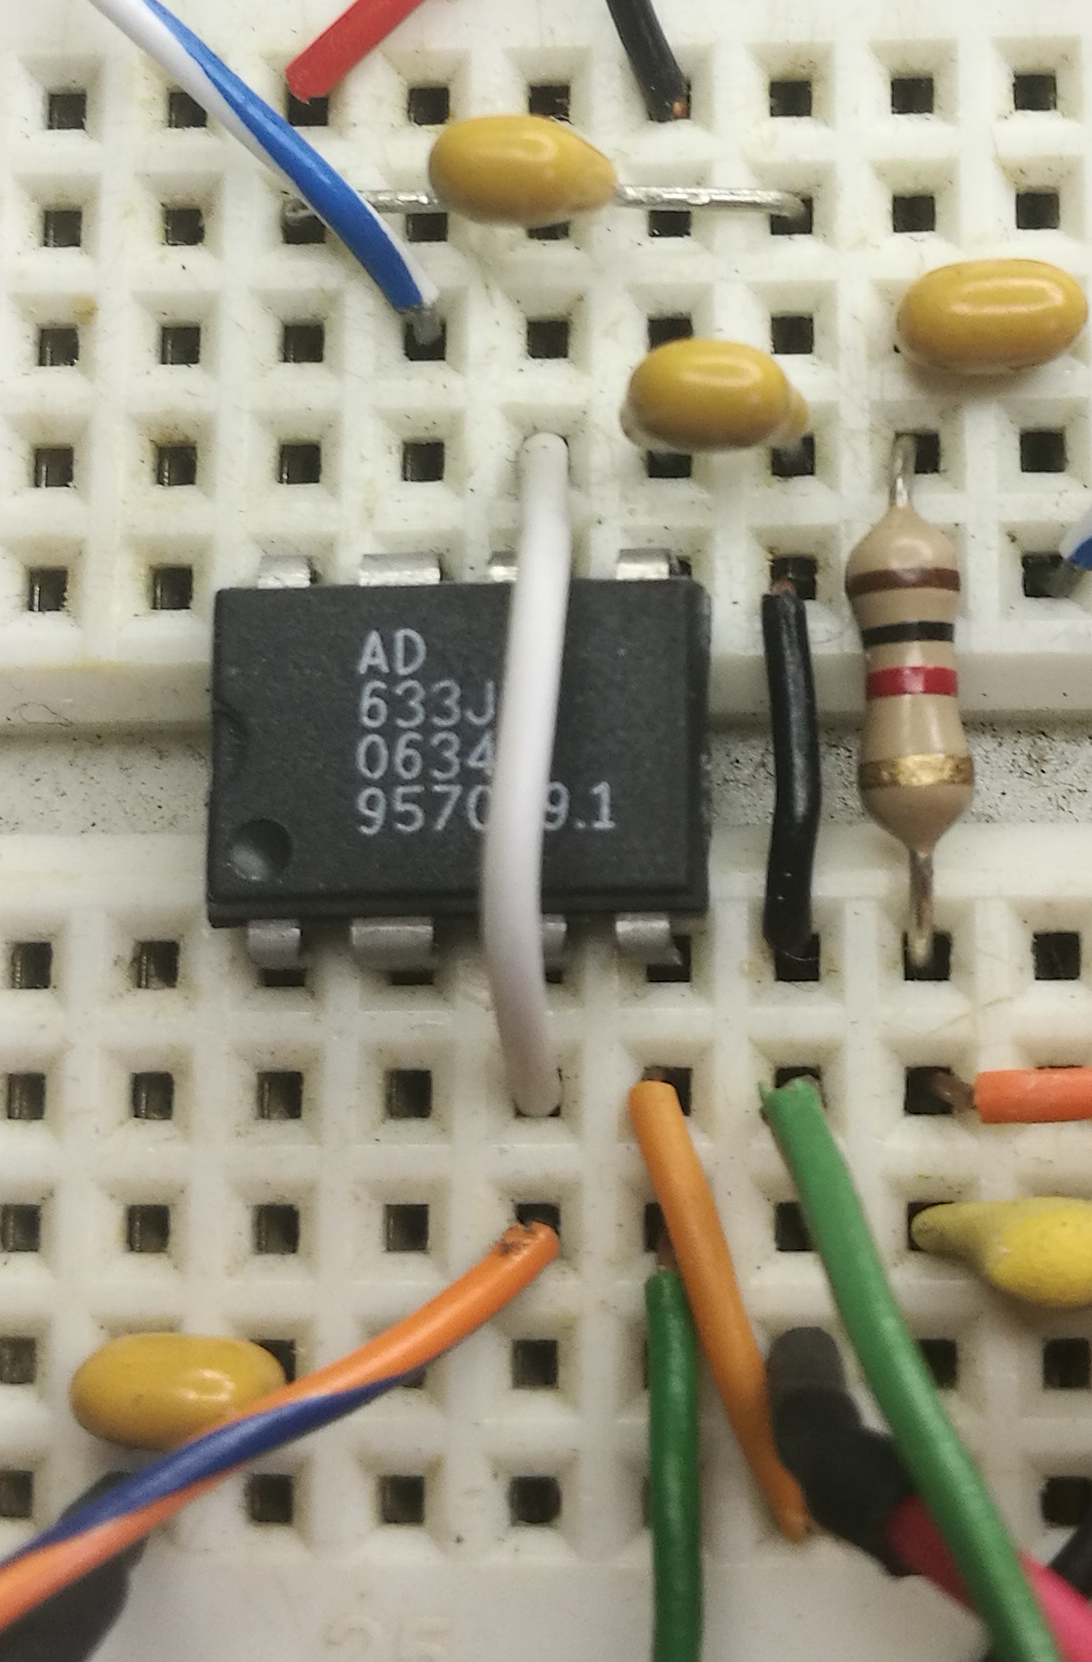
\includegraphics[width=0.3\textwidth]{Figures/Implementation/Mixer/mixerbboard.png}
    \caption{AM mixer implemented on breadboard}
    \label{fig:mixerbb}
\end{figure}

A test tone of 2.5 kHz is generated and input as the modulating waveform with a 40 kHz carrier input to the AD633 AM modulator and the outputs are shown in figure \ref{fig:mix2.5kinputVsOut} and \ref{fig:mix40kinputVsOut}.

\begin{figure}[ht!]
\centering

    \begin{minipage}{0.49\textwidth}
    \centering
    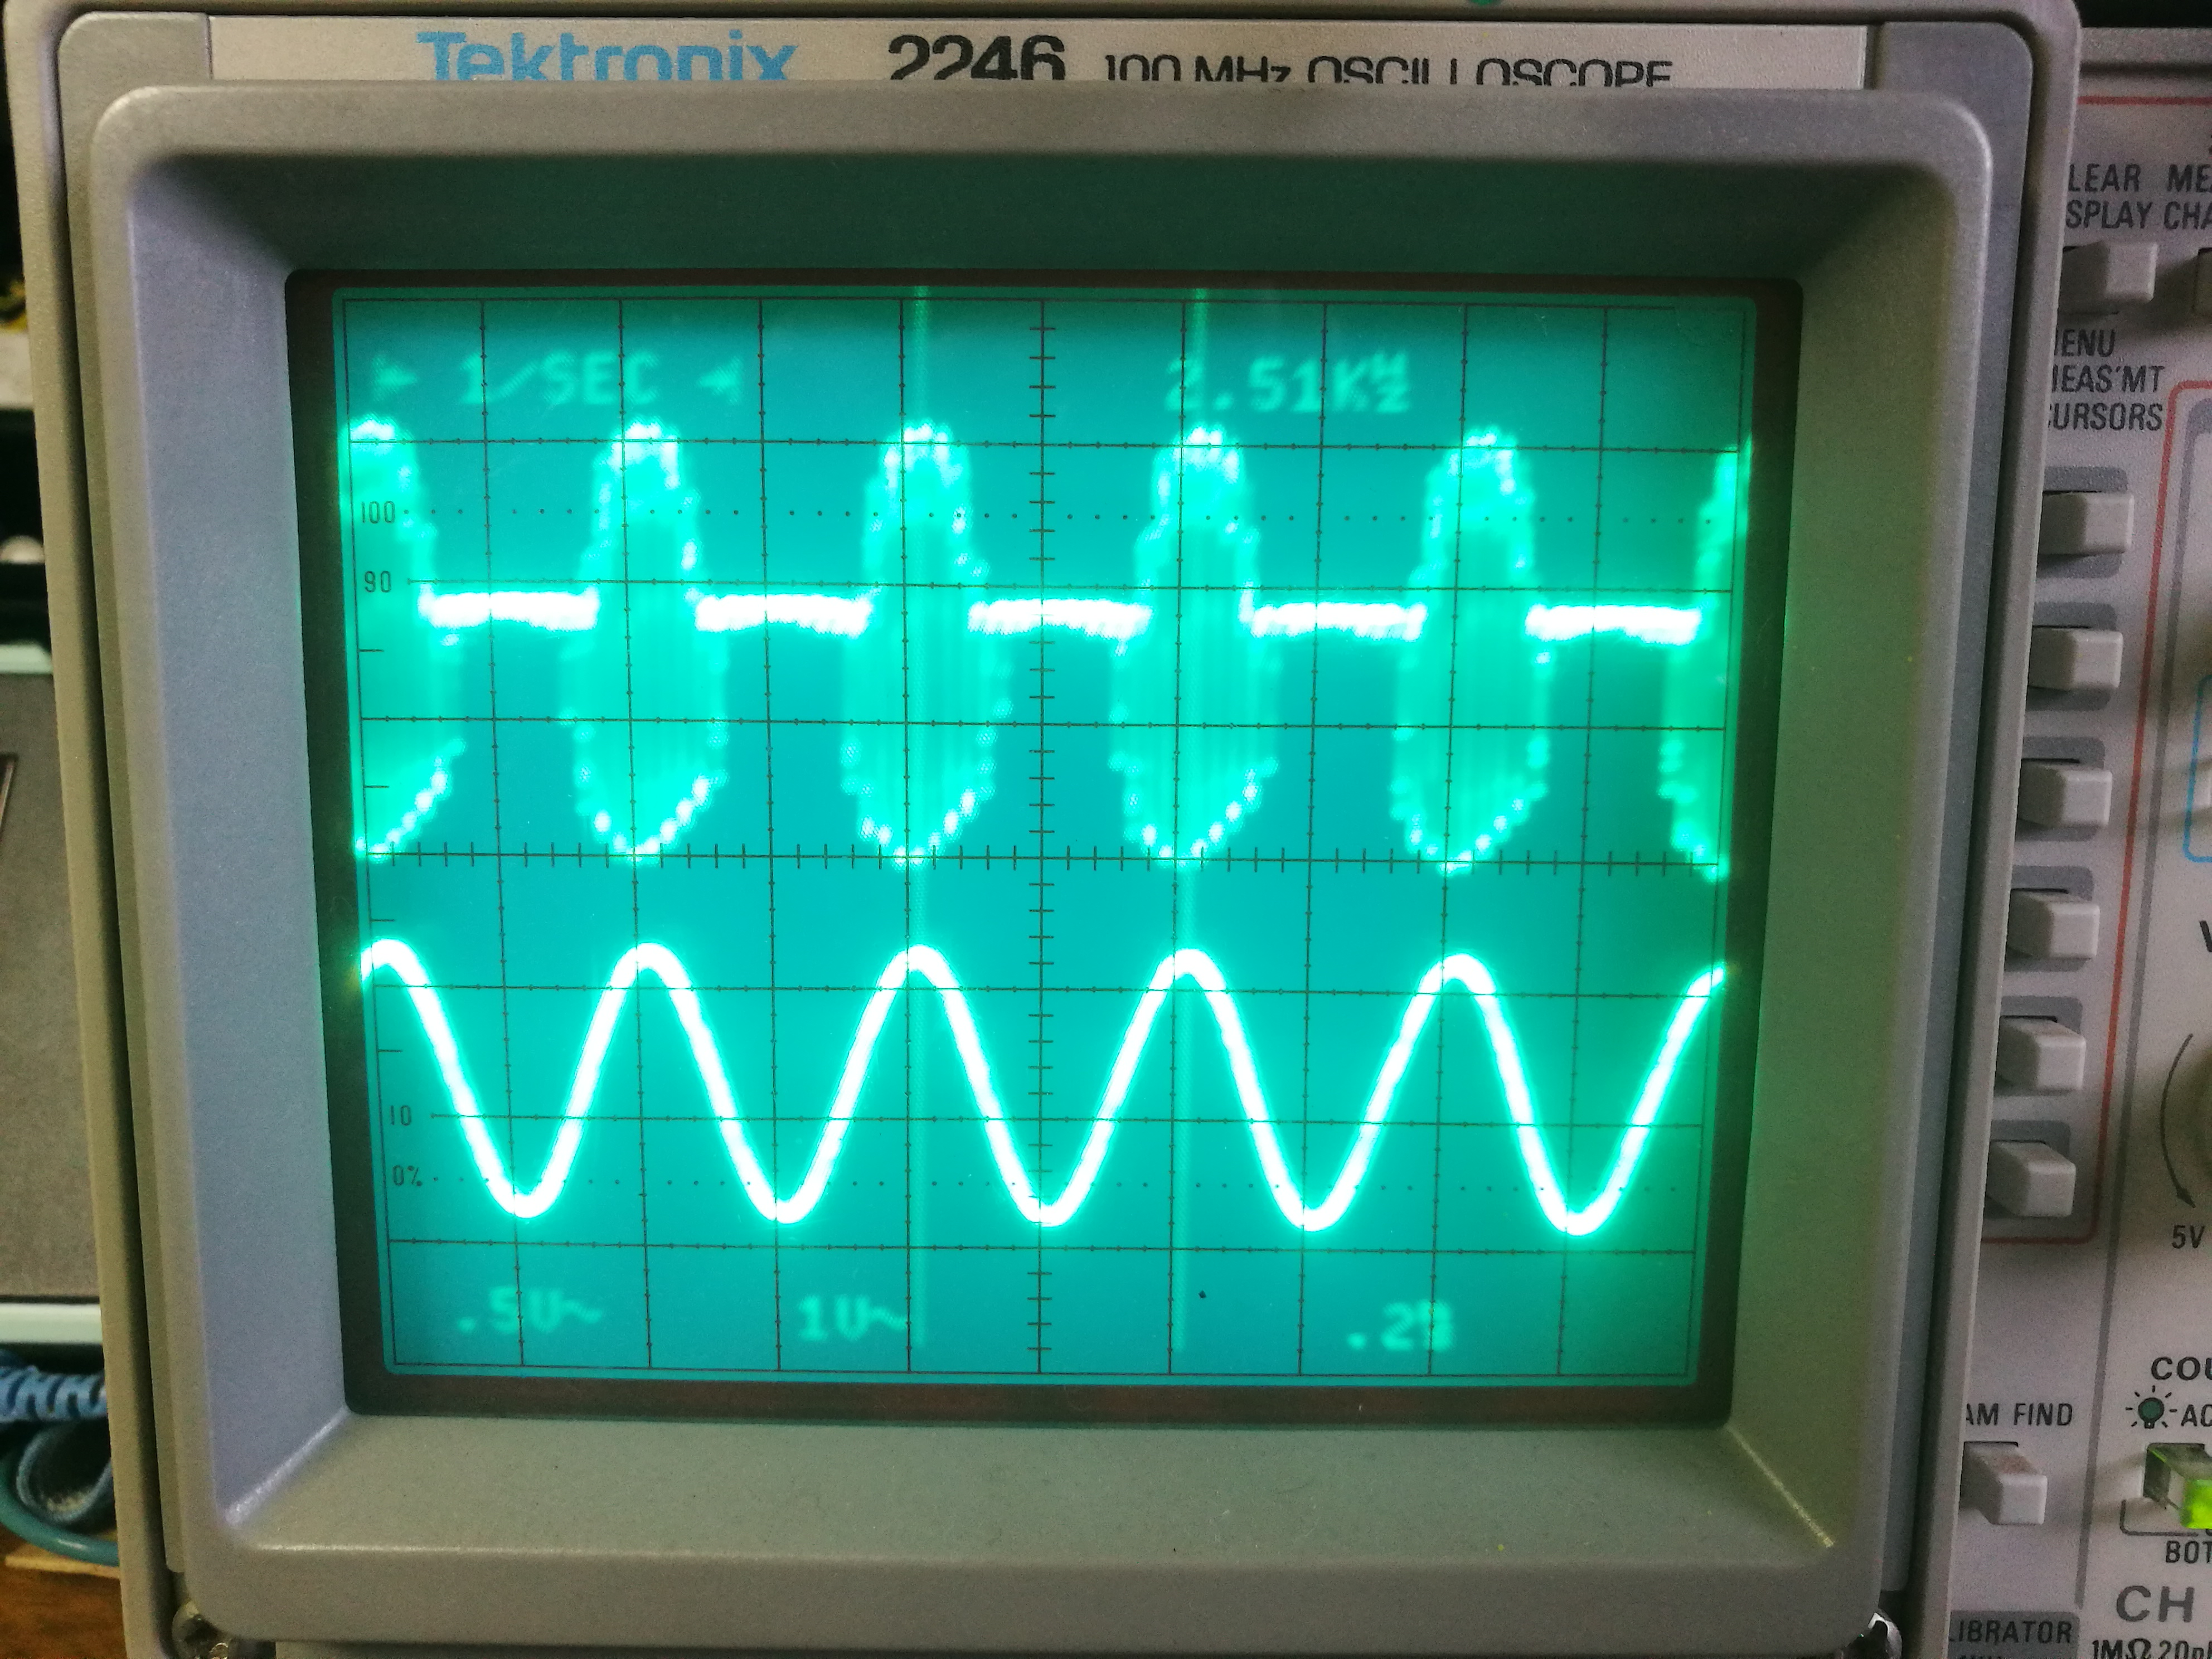
\includegraphics[width= \textwidth]{Figures/Implementation/Mixer/infreq.jpg}
    \caption{Input 2.5 kHz frequency compared to modulated output}
    \label{fig:mix2.5kinputVsOut}
    \end{minipage}\hfill
    \begin{minipage}{0.49\textwidth}
    \centering
    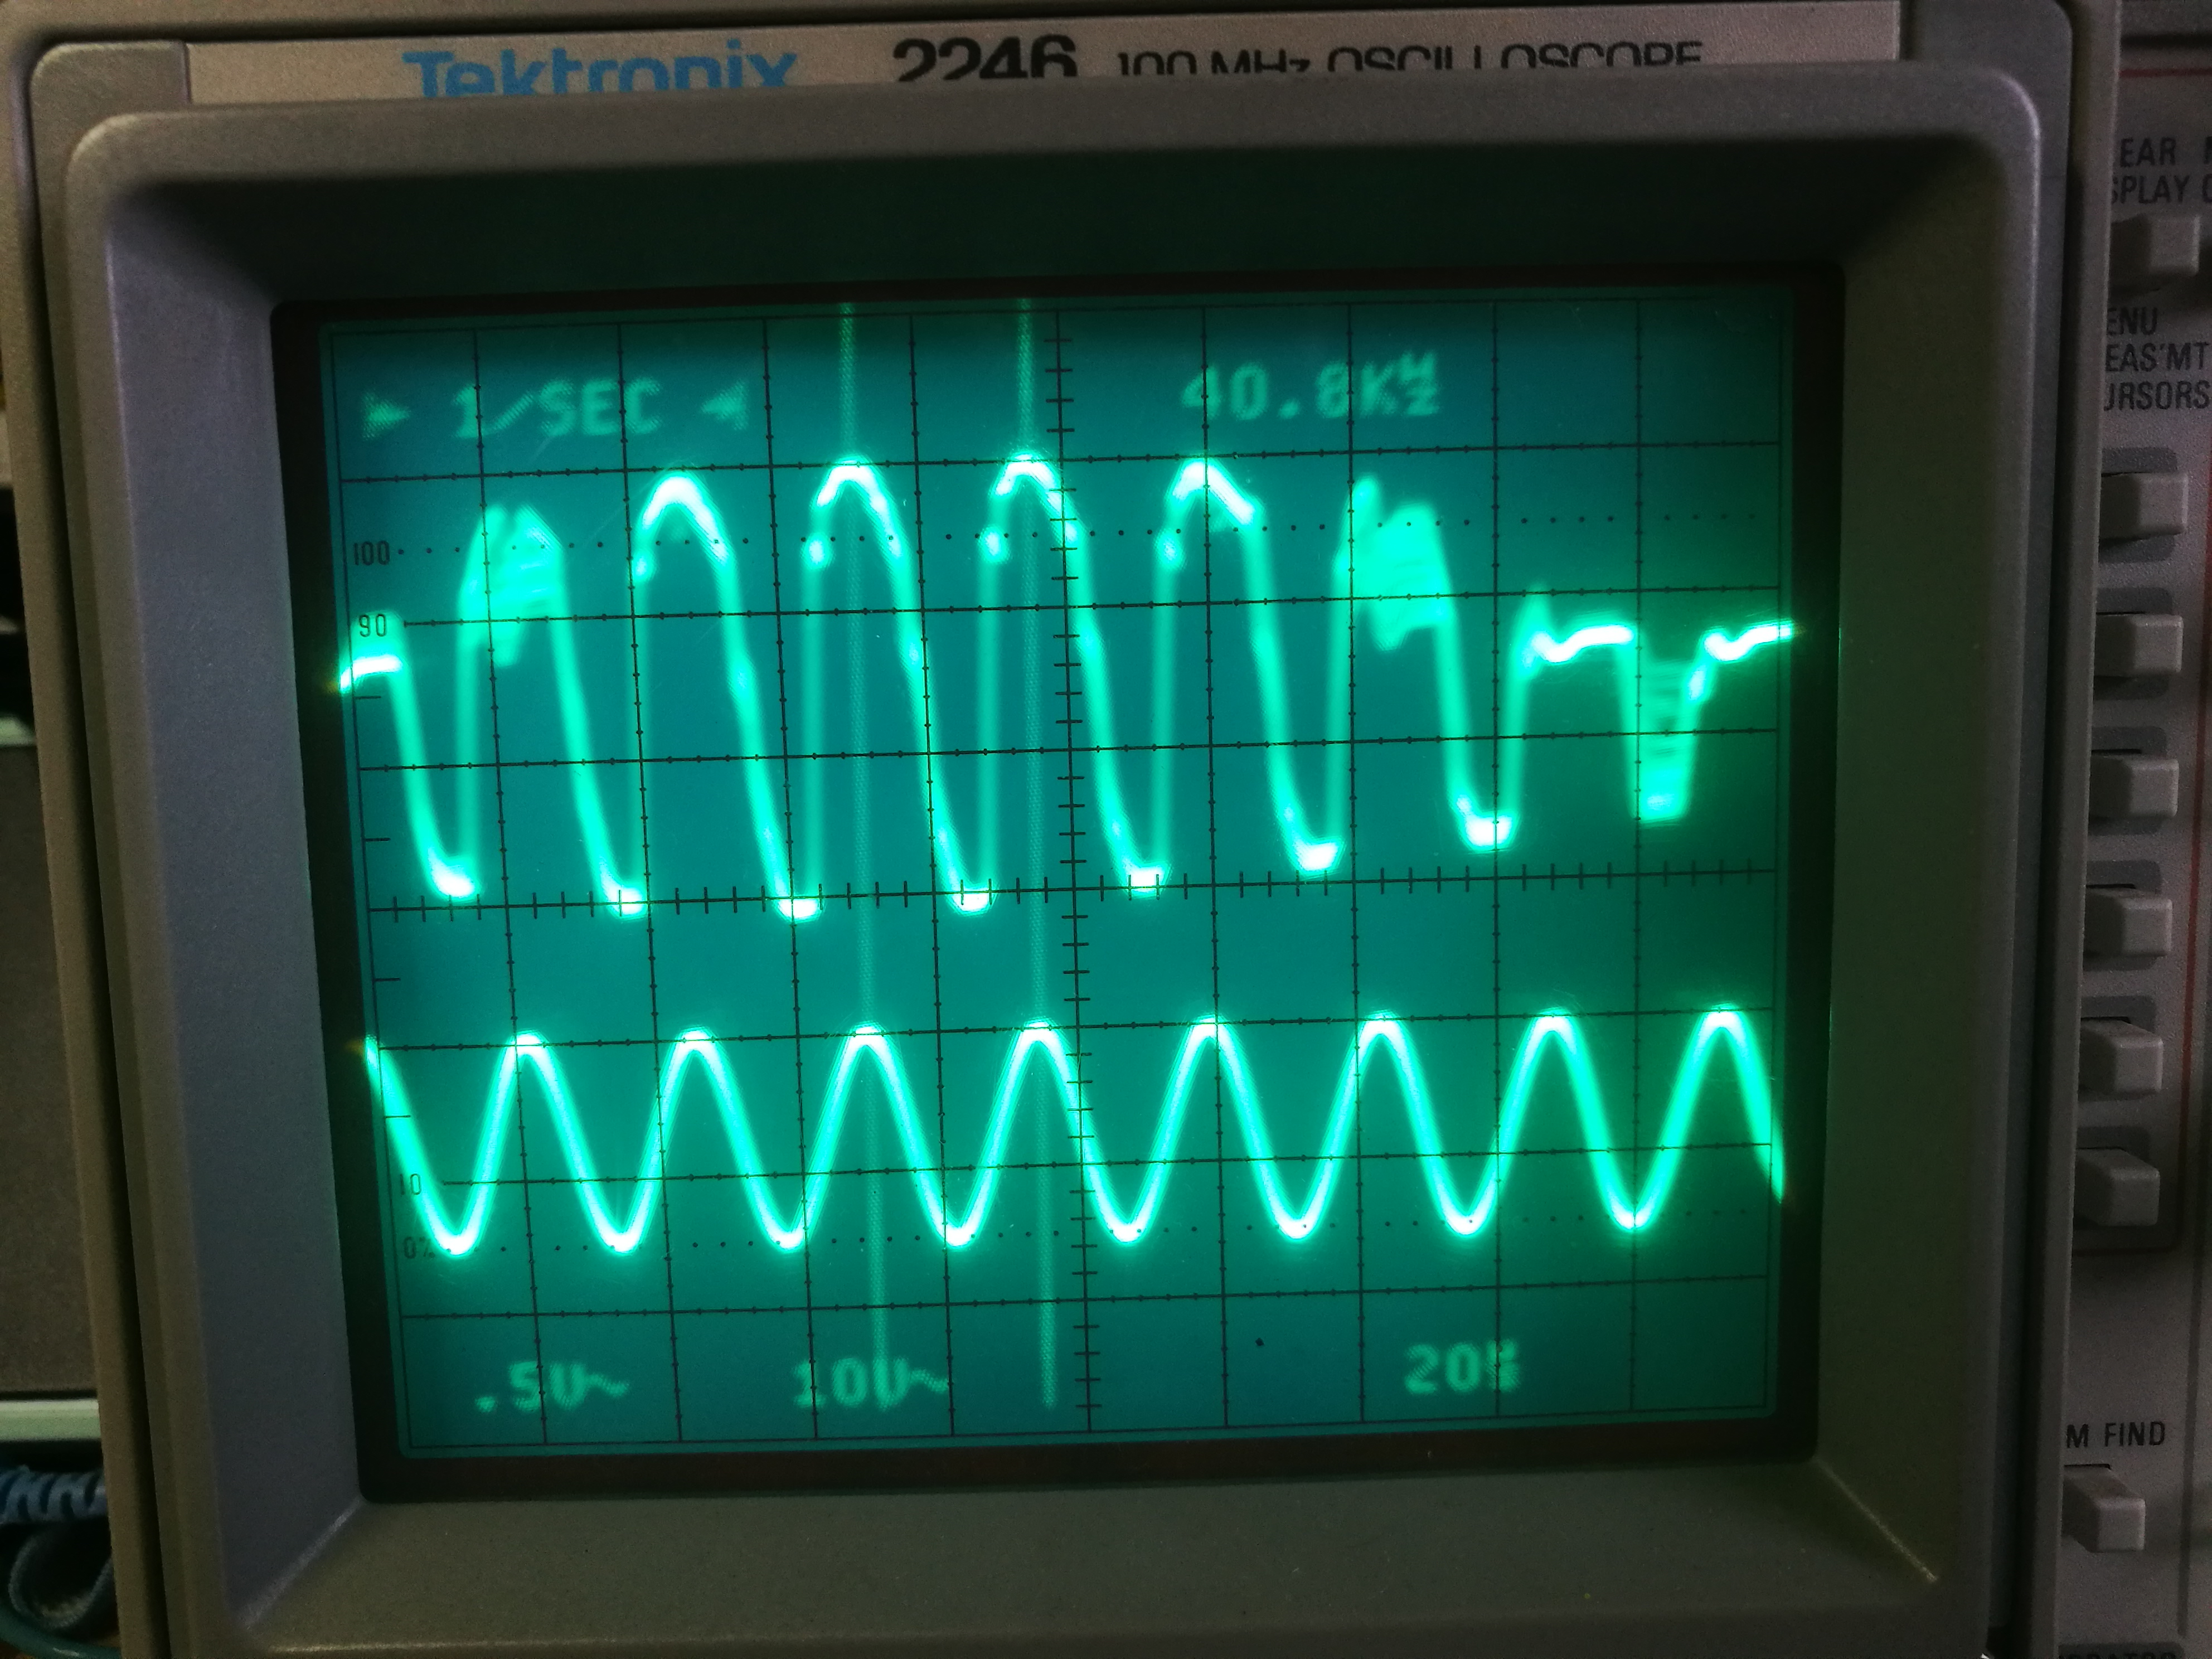
\includegraphics[width= \textwidth]{Figures/Implementation/Mixer/outfreq.jpg}
    \caption{Input 40 kHz frequency compared to modulated output}
    \label{fig:mix40kinputVsOut}
    \end{minipage}
    
\end{figure}

Figure \ref{fig:mixerinVsout} demonstrates the input modulating signal compared to the output AM signal. The output shows an approximate peak amplitude of 1.5V with a near zero amplitude for the negative half cycle. While this doesn't match up well with the expected output levels of the simulations; it is still an acceptable result for the subsystem. From these measurements the modulation index appears to lie around 50\% using equation \ref{eqn:modIndex} given a carrier amplitude of 1V.

\begin{figure}[ht!]
    \centering
    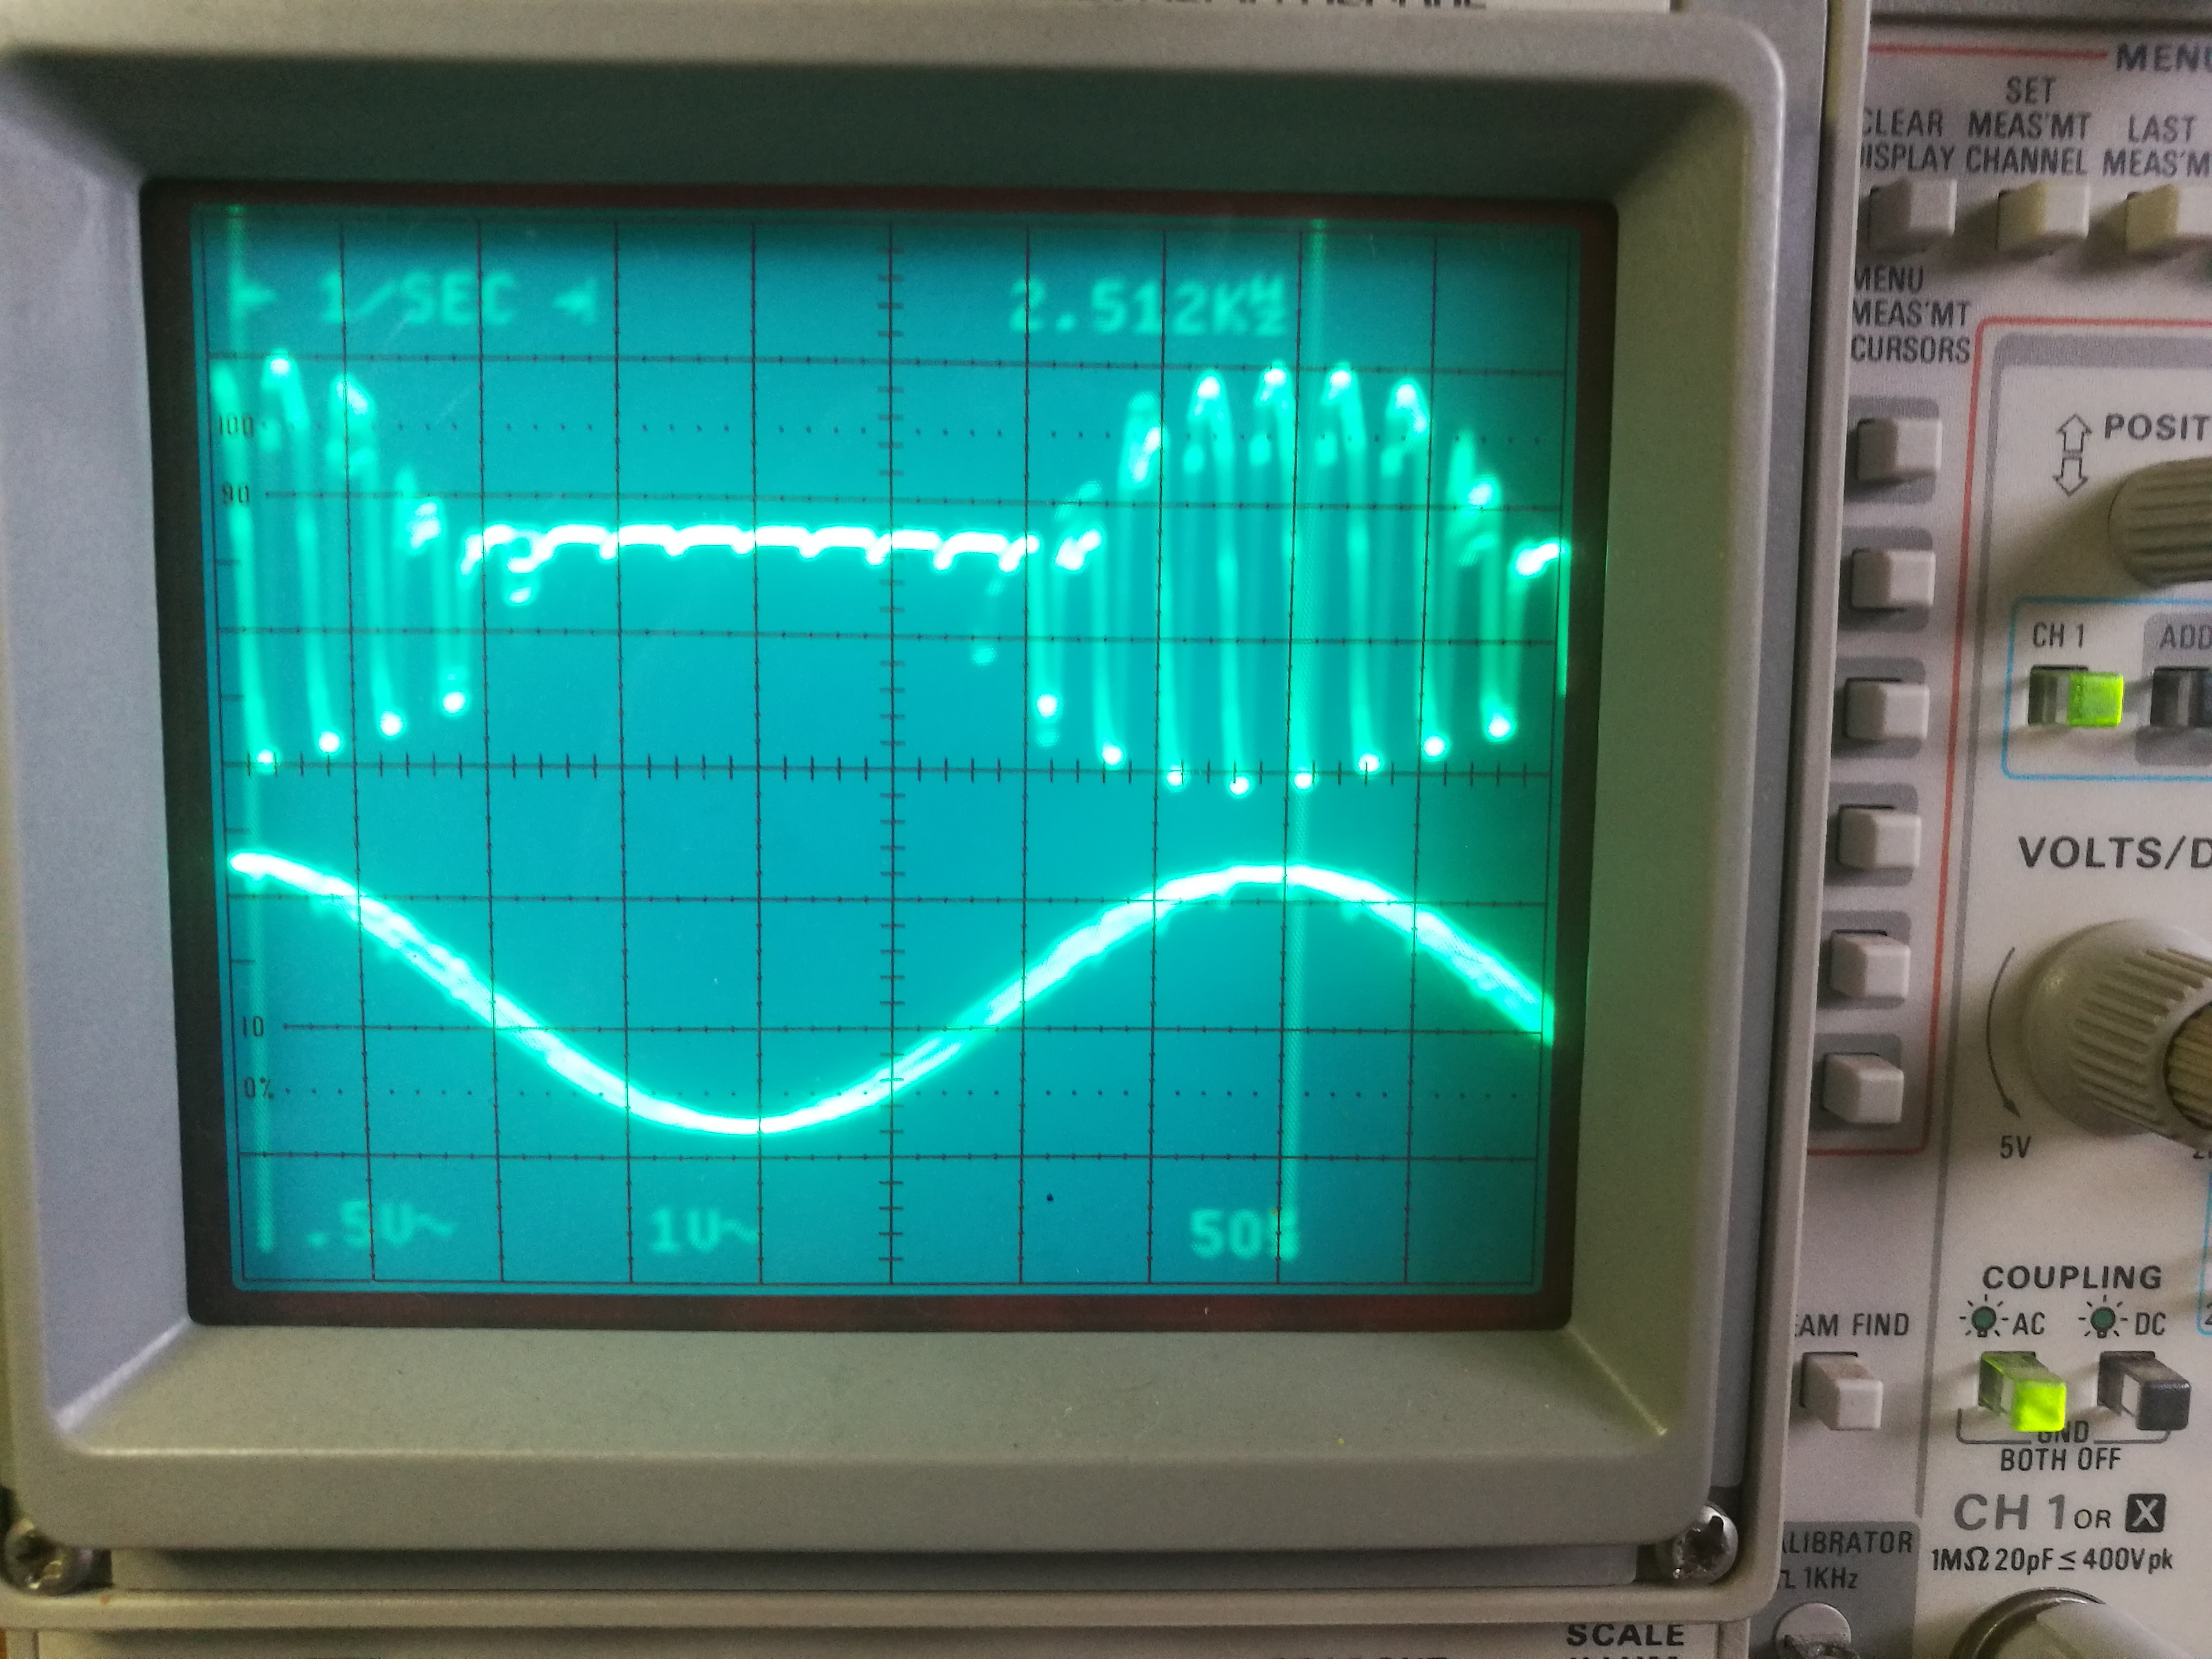
\includegraphics[width=0.8\textwidth]{Figures/Implementation/Mixer/mixoutVsin.jpg}
    \caption{AM mixer output versus input signal}
    \label{fig:mixerinVsout}
\end{figure}

\subsubsection{Amplifier Implementation}
The implementation of the amplifier involved many small tweaks from the original design due to a low frequency oscillations occurring on the output. As such the final implementation involves many more components that were used to reduce these low frequency oscillations during the troubleshooting process. Figure \ref{fig:ampbbCirc} demonstrates the end result from the troubleshooting where the oscillations were under control. Figure \ref{fig:ampCircPosttbl} illustrates the new circuit after troubleshooting the low frequency oscillations.

\begin{figure}[ht!]
    \centering
    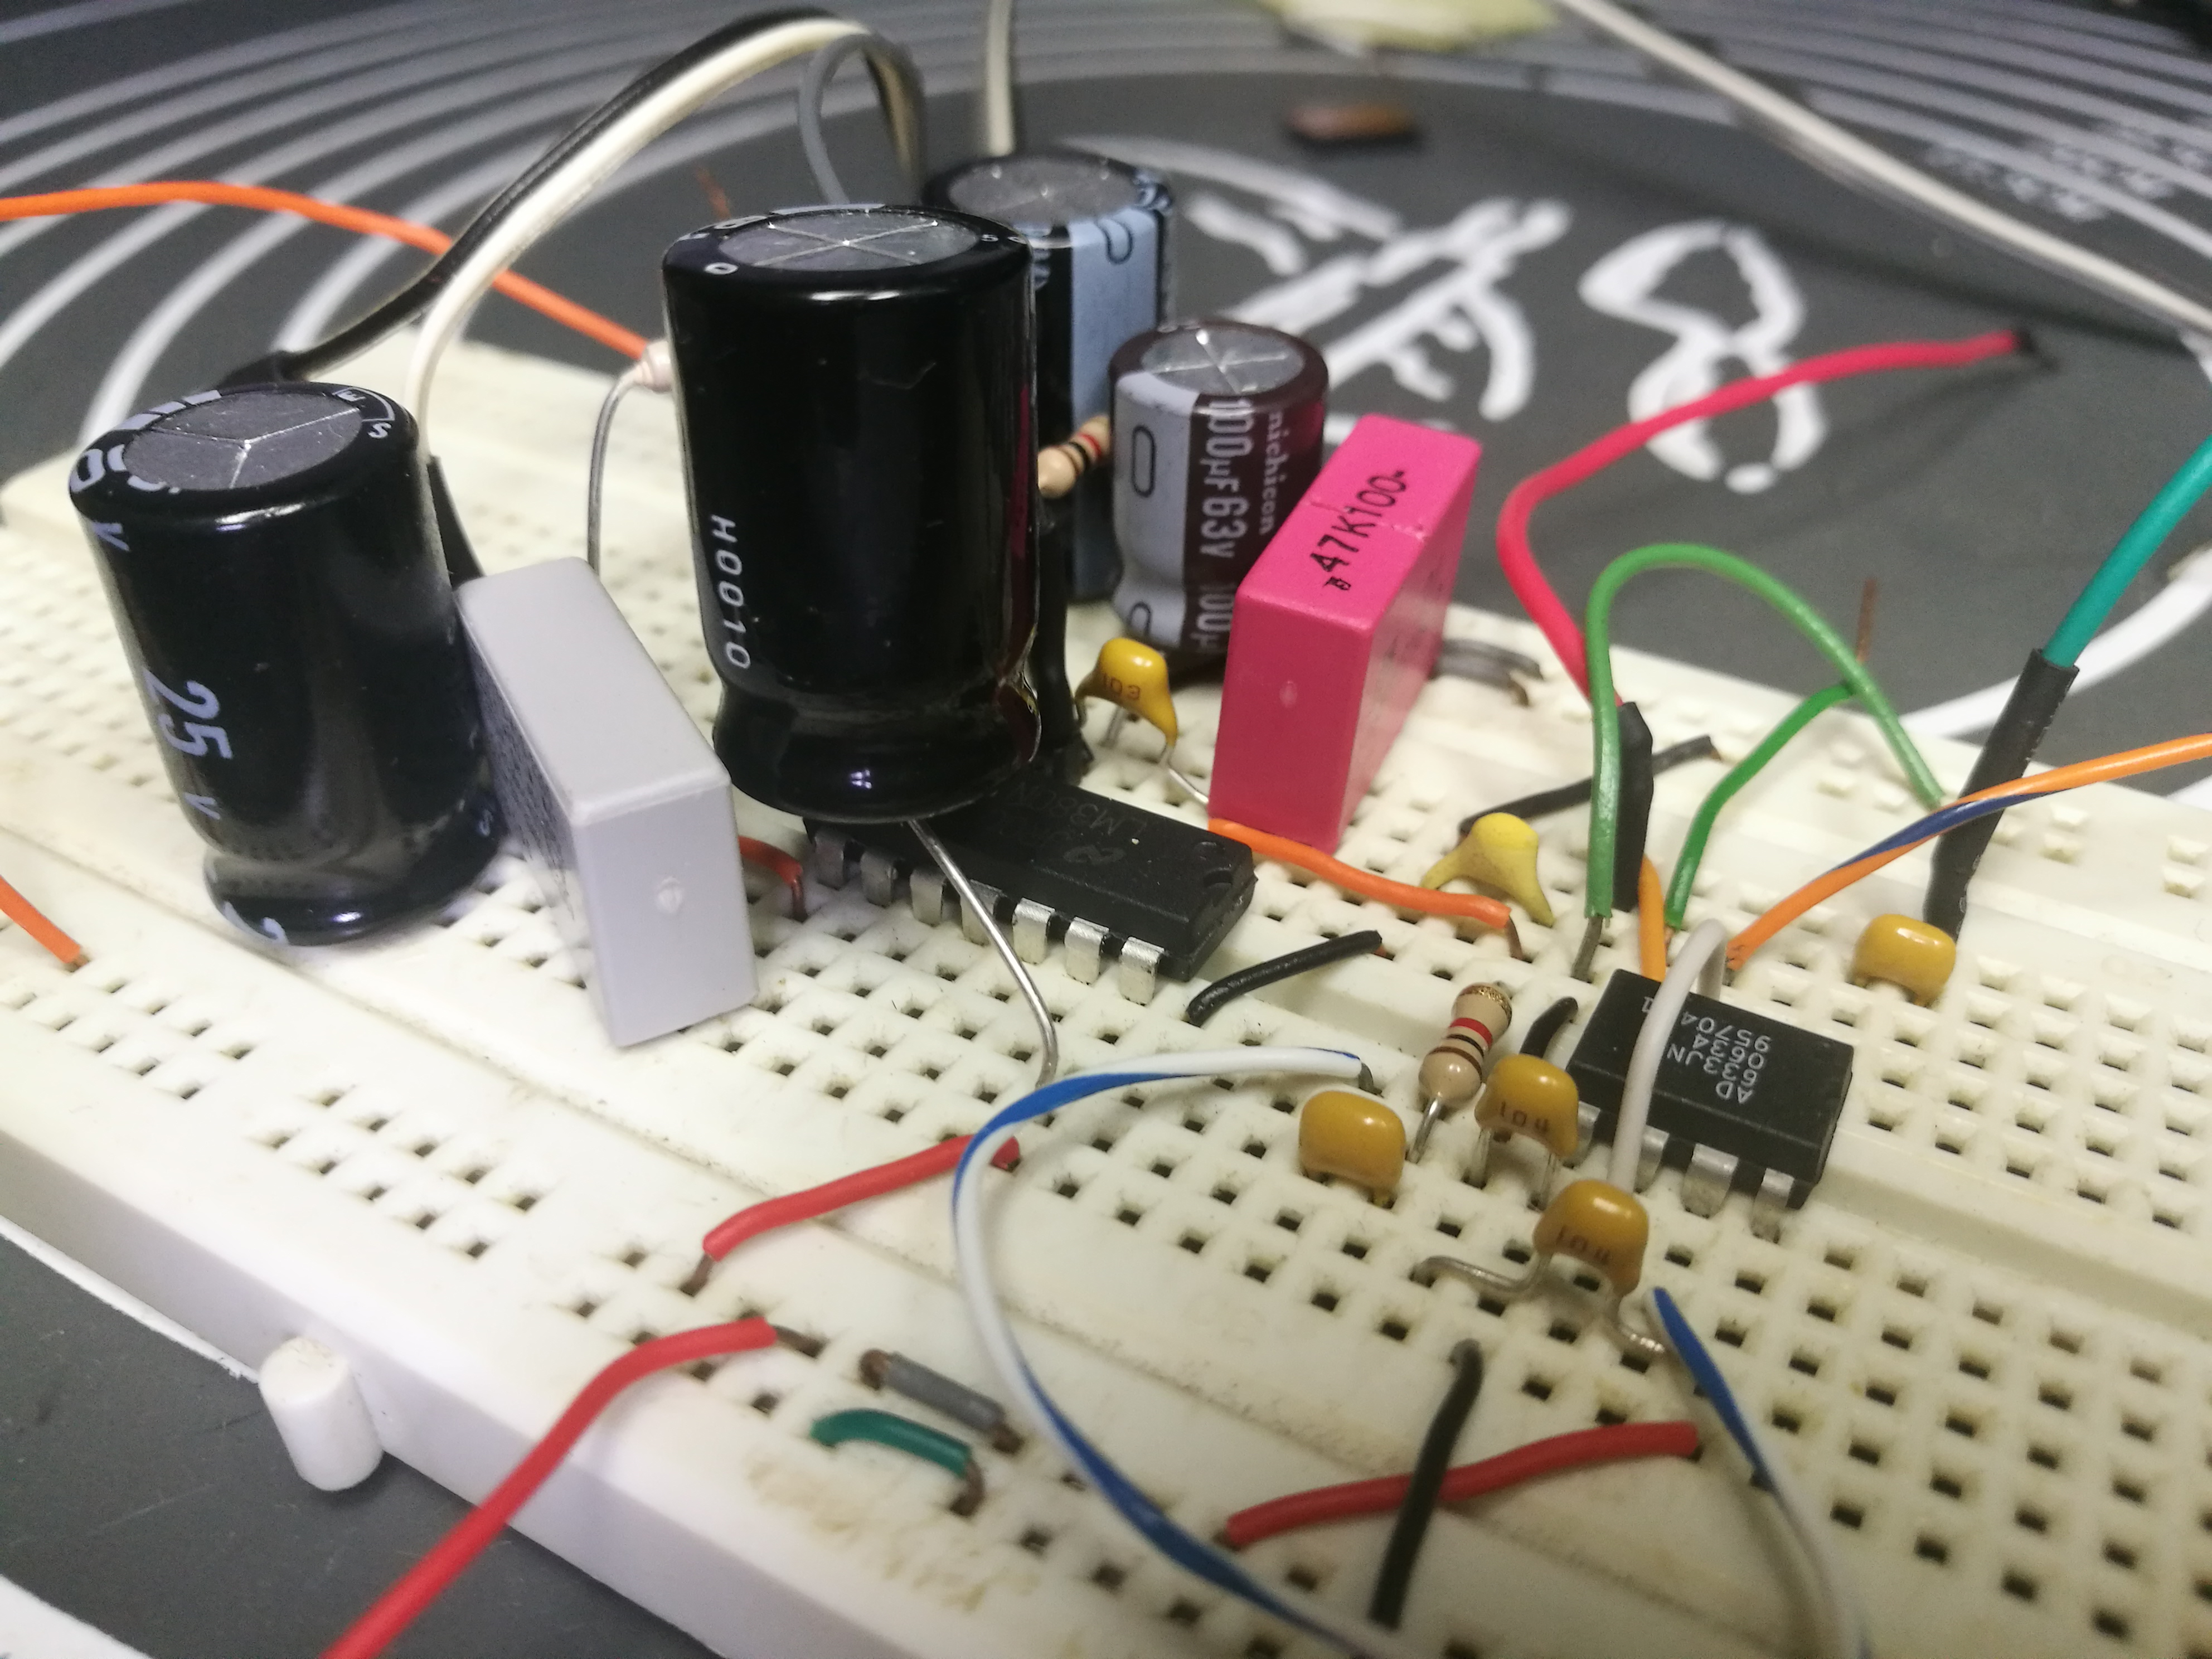
\includegraphics[width=0.8\textwidth]{Figures/Implementation/Amplifier/ampbbcirc.jpg}
    \caption{LM380 Power amplifier breadboard circuit after troubleshooting}
    \label{fig:ampbbCirc}
\end{figure}

\begin{figure}[ht!]
    \centering
    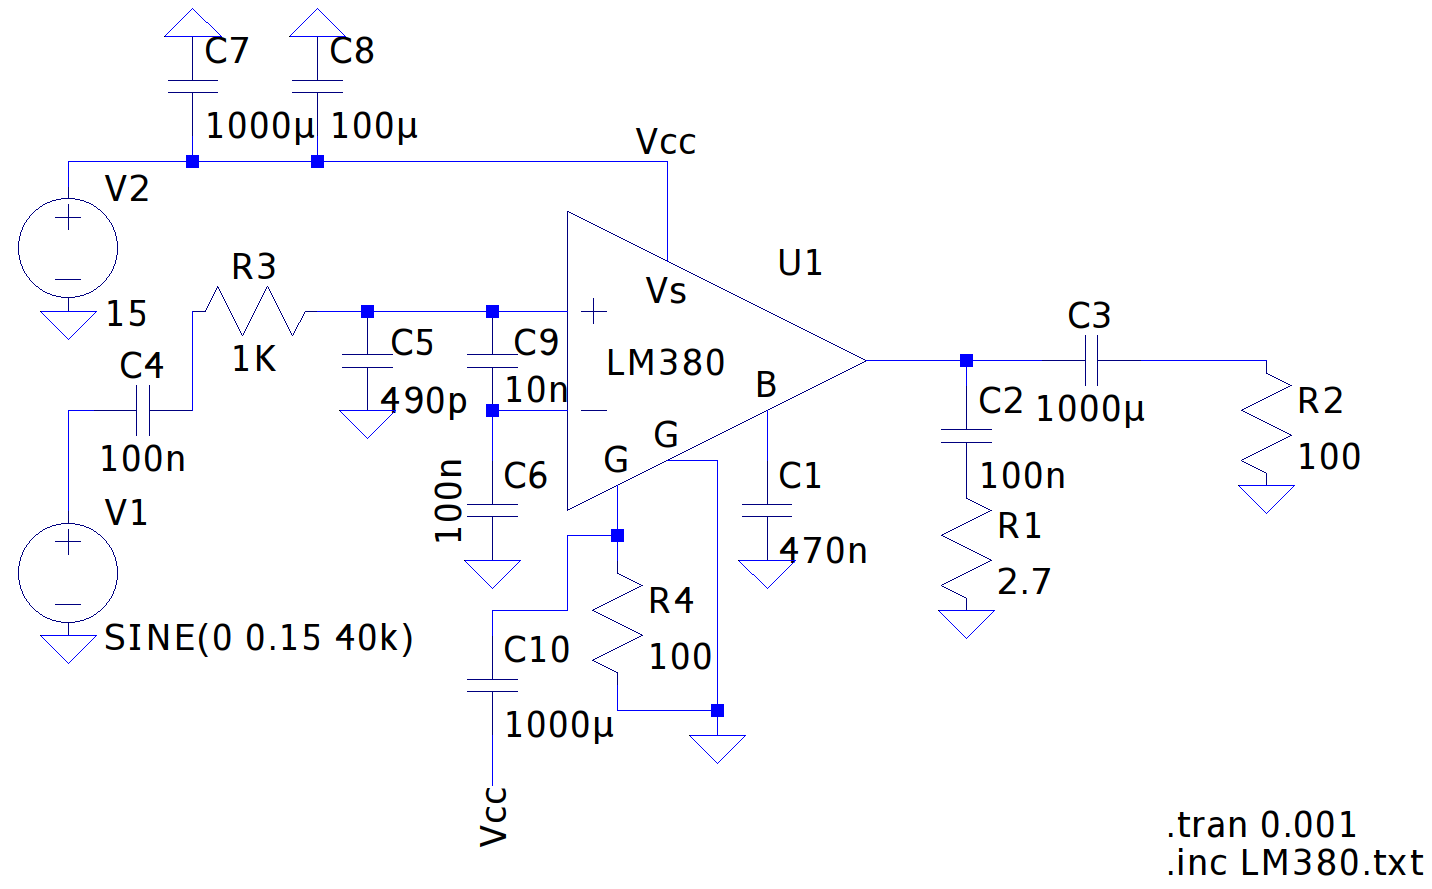
\includegraphics[width=0.8\textwidth]{Figures/Implementation/Amplifier/Lm380Mod.png}
    \caption{LM380 Power amplifier circuit schematic after troubleshooting}
    \label{fig:ampCircPosttbl}
\end{figure}

Upon application of a low frequency test tone of 500 Hz to a ordinary speaker, the amplifier produced an audible output with no low frequency oscillations. The output shown in figure \ref{fig:ampOscOut} demonstrates the resultant output of the amplifier. The output only shows the positive half cycle of the wave due to the electrolytic capacitor present on the output, blocking the negative half cycle. Unfortunately no alternative capacitors were readily available to correct this since the restrictions imposed by Covid-19 blocked access to components.
\begin{figure}[ht!]
    \centering
    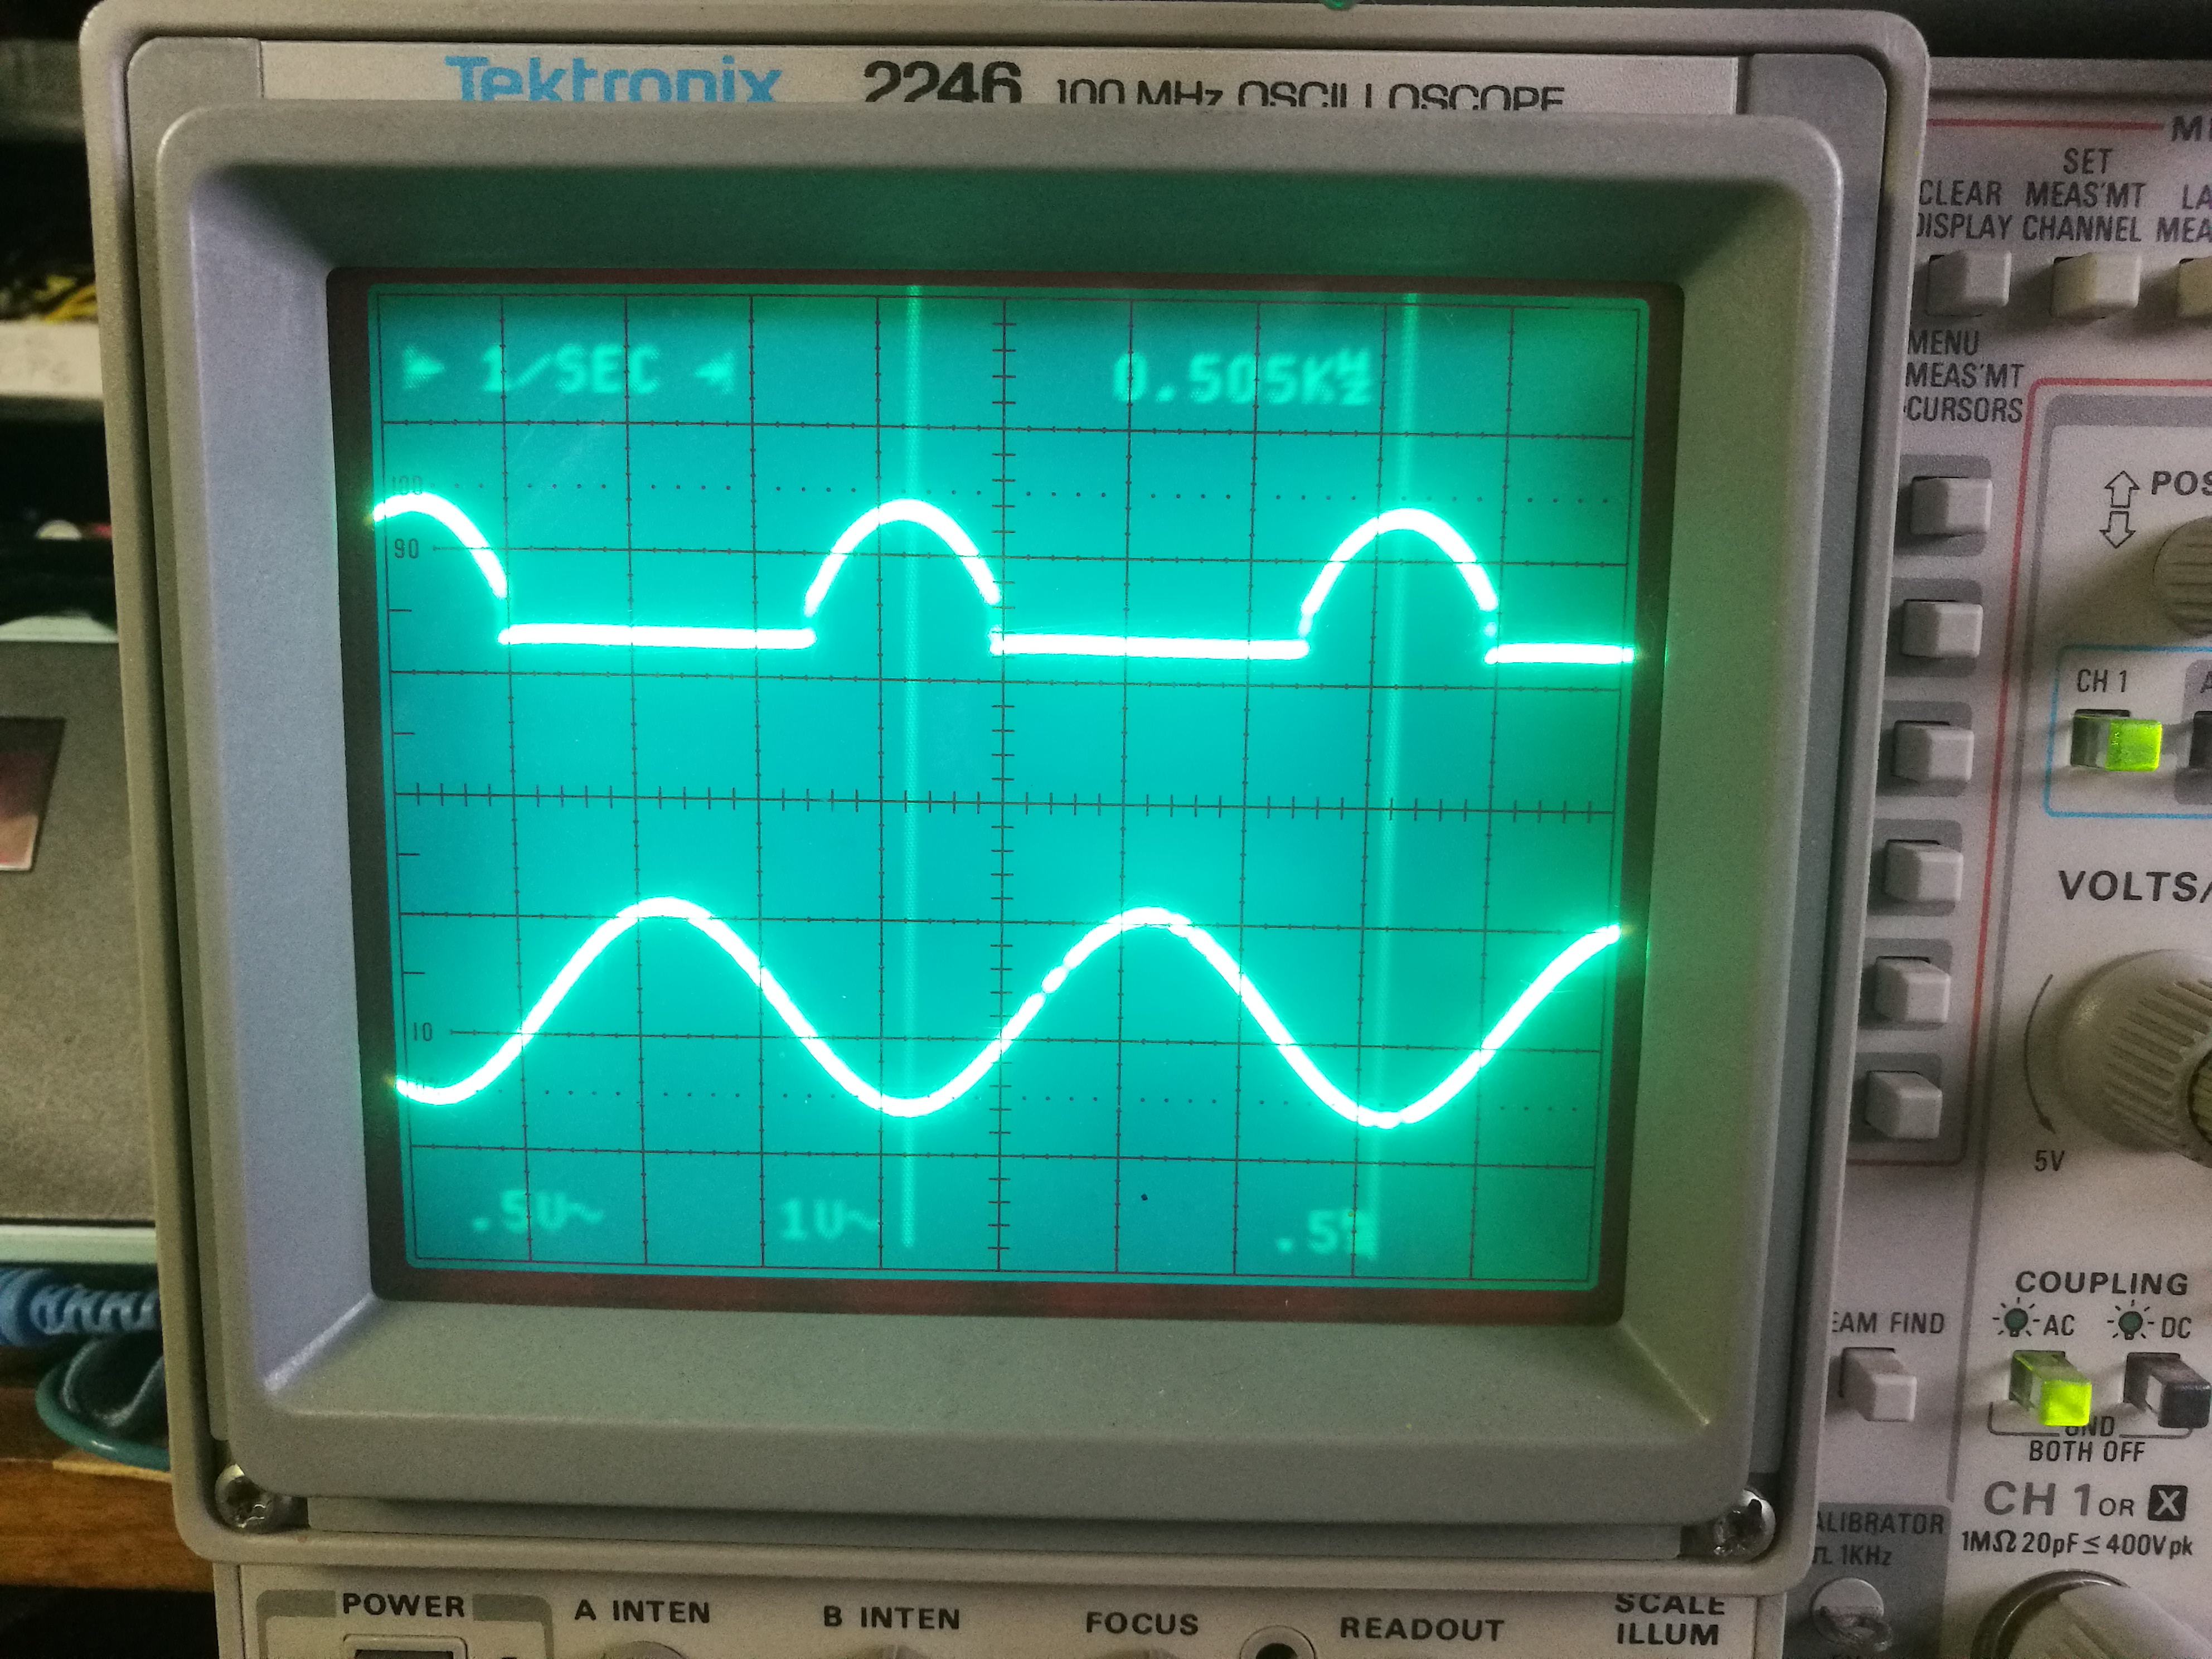
\includegraphics[width=0.8\textwidth]{Figures/Implementation/Amplifier/ampOutbb.jpg}
    \caption{LM380 Power amplifier 500 Hz output to test speaker}
    \label{fig:ampOscOut}
\end{figure}
Since the capacitor's main purpose is to smooth out the peeks for the 8 $\Omega$ speaker during this test, it can be bypassed when connecting the ultrasonic array.

\subsection{Transducer array construction}
The construction of the transducer array began once the previously designed PCBs arrived from JLC PCB. 21 Kibitone 400ST ultrasonic transducers were placed into the spaces provided by the PCB paying careful attention transducer orientation and soldered in place. Once soldered, a 40 kHz tone was generated by the function generator and attached to the input of the PCB. Using 2 channels on a Tektronix 2246 oscilloscope, a receiver transducer was attached to one probe while the other probe was attached to the PCB input signal allowing the output ultrasonic waves to be analysed and tested for any faults. The receiver transducer was passed over each emitting transducer and compared to the input signal, this test resulted in two transducers (BZ7 and BZ17 on the PCB) producing a $180^\circ$ phase shifted output as shown in figure 


\subsection{Pre-processing development}

